\documentclass[a4paper,12pt]{article}
\usepackage[utf8]{inputenc}
\usepackage[T1]{fontenc}
\usepackage{geometry}
\geometry{top=3cm,bottom=2cm,left=3cm,right=2cm}
\usepackage{parskip}
\usepackage{enumitem}
\usepackage{titlesec}
\usepackage{tocloft}
\usepackage{setspace}
\usepackage{lmodern}
\usepackage{indentfirst}
\usepackage{svg}
\usepackage{caption}
\usepackage{hyperref}
\hypersetup{colorlinks=true,linkcolor=black,urlcolor=blue}
\usepackage{helvet} % Use Helvetica (Arial equivalent)
\renewcommand{\familydefault}{\sfdefault} % Set default font to sans-serif (Arial-like)
\usepackage{fancyhdr} % Pacote para personalizar cabeçalhos e rodapés
\usepackage{graphicx} % Add this line to include the graphicx package
\usepackage{url} % Add this line to include the url package

\setstretch{1.5}

\titleformat{\section}{\normalfont\bfseries\uppercase}{\thesection}{1em}{}
\titleformat{\subsection}{\normalfont\bfseries}{\thesubsection}{1em}{}
\titleformat{\subsubsection}{\normalfont\itshape}{\thesubsubsection}{1em}{}

\renewcommand{\cftsecfont}{\normalfont}
\renewcommand{\cftsecpagefont}{\normalfont}
\renewcommand{\cftsecleader}{\cftdotfill{\cftdotsep}}

\renewcommand{\contentsname}{Sumário}

\fancypagestyle{plain}{
    \fancyhf{} % Limpa os cabeçalhos e rodapés
    \fancyfoot[R]{\thepage} % Adiciona a numeração no canto inferior direito
    \renewcommand{\headrulewidth}{0pt} % Remove a linha do cabeçalho
    \renewcommand{\footrulewidth}{0pt} % Remove a linha do rodapé
}

\begin{document}

\pagestyle{fancy}
\fancyhf{} % limpa cabeçalho e rodapé
\fancyfoot[R]{\thepage} % número da página no rodapé direito
\renewcommand{\headrulewidth}{0pt} % remove linha do cabeçalho
\renewcommand{\footrulewidth}{0pt} % remove linha do rodapé

% Capa
\begin{titlepage}
    \centering
    
\includegraphics[width=0.8\textwidth]{unip-logo.pdf}
    \vspace*{2cm}
    {\normalfont\bfseries\LARGE MYSUPPORT AI \par}
    \vspace{1cm}
    {\large Projeto para suporte ao usuário em software e hardware com IA \par}
    \vspace{1cm}
    {\large LIMEIRA \par}
    \vspace{0.5cm}
    {\large 2025 \par}
    \vspace{2cm}
    {\normalsize
        Andrew Stewart Grama Rodini \par
        Guilherme Aparecido Mariano \par
        Jesse Viana Gusmão \par
        Leonardo Bertolo Armbruster \par
        Luis Guilherme Alves De Oliveira \par
        Rafael Dias De Argolo \par
        Rafael Guilherme Treffet Allegri \par
    }
    \vspace{2cm}
    {\large Projeto Integrador apresentado como parte dos requisitos de avaliação do 3º semestre do curso de Análise e Desenvolvimento de Sistemas (ADS). \par}
    \vspace{1cm}
    \vspace{9cm}
    {\large LIMEIRA \par}
    \vspace{0.5cm}
    {\large 2025 \par}
\end{titlepage}

% Folha de rosto
\begin{titlepage}
    \centering
    \vspace*{2cm}
    {\normalfont\bfseries\LARGE MYSUPPORT AI \par}
    \vspace{1cm}
    {\large Projeto para suporte ao usuário em software e hardware com IA \par}
    \vspace{2cm}
    {\normalsize
        Trabalho apresentado ao curso de Análise e Desenvolvimento de Sistemas (ADS) da Faculdade UNIP, como requisito parcial para obtenção de nota na disciplina de Projeto Integrador. \par
    }
    \vspace{1cm}
    {\normalsize Orientadora: Profª Sandra \par}
    \vspace{9cm}
    {\large LIMEIRA \par}
    \vspace{0.5cm}
    {\large 2025 \par}
\end{titlepage}

% Sumário
\tableofcontents
\newpage

% Corpo do texto
\section{INTRODUÇÃO}
Apresentaremos neste trabalho um chat com assistência de IA voltado para o mundo da tecnologia em geral, auxiliando o usuário que não possui conhecimento específico referente a hardware e software. O objetivo é buscar a resolução de problemas de forma mais rápida e eficiente para um usuário inexperiente, otimizando o tempo e facilitando o processo.

\section{APRESENTAÇÃO DO PROJETO}
MySupport AI é um assistente web voltado para solucionar problemas ou dúvidas de usuários em geral, visando facilitar e agilizar o compartilhamento de soluções.

\section{ESCOPO DO PROJETO}
Desenvolver um sistema de inteligência artificial que ofereça atendimento automatizado e eficiente aos clientes, com capacidade de resolver dúvidas frequentes, encaminhar solicitações e aprender com interações anteriores.

\section{INFRAESTRUTURA}
\subsection{EQUIPAMENTOS}
\begin{itemize}
    \item Servidores para hospedagem da aplicação
    \item Computadores (desktop e laptops) para atendimento e operação
    \item Dispositivos móveis (tablets e smartphones) para acesso remoto
    \item Equipamentos de rede (roteadores, switches, modems)
    \item Ferramentas de Backup de dados e redundância
    \item Dispositivos de segurança (firewalls, antivírus, câmeras de segurança)
\end{itemize}
\clearpage

\subsection{SERVIDOR}
\begin{itemize}
    \item Servidores web para processamento das solicitações de suporte
    \item Bancos de dados relacionais para armazenamento de informações de usuários e históricos de interação
    \item Ferramentas de análise de dados para monitoramento em tempo real e melhoria contínua do suporte
    \item Sistemas de segurança para proteger dados sensíveis e garantir a privacidade
    \item Ferramentas de integração com plataformas de terceiros (CRM, APIs de chat, etc.)
\end{itemize}

\section{DESCRIÇÃO GERAL DO PRODUTO}
O sistema de suporte com IA é uma plataforma web desenvolvida para otimizar o atendimento ao cliente, integrando inteligência artificial para respostas automatizadas e triagem de chamados. A aplicação permite o gerenciamento eficiente de tickets, histórico de atendimentos e interação em tempo real com os usuários.

\section{FUNÇÕES DO PRODUTO}
\begin{itemize}
    \item Atendimento Automatizado: Respostas instantâneas a perguntas frequentes utilizando IA.
    \item Gestão de Chamados: Criação, acompanhamento e resolução de tickets de suporte.
    \item Histórico de Atendimentos: Registro detalhado das interações com os clientes.
    \item Chat em Tempo Real: Comunicação direta entre clientes e equipe de suporte.
    \item Painel Administrativo: Dashboard para monitoramento de métricas e desempenho do suporte.
\end{itemize}

\section{INTERFACES DE USUÁRIO}
A interface do sistema de suporte com inteligência artificial é centrada em um chatbot interativo. A tela principal contém uma área de conversa onde o usuário digita e recebe mensagens em tempo real, acompanhada de um campo de entrada e botão de envio. O assistente virtual responde de forma clara e objetiva, com opções de respostas rápidas para facilitar o uso. Também há a opção de envio de fotos para solucionar erros com mais facilidade.

\section{INTERFACES DE HARDWARE}
Para o melhor funcionamento e otimização de tempo temos como aliados nossos sistemas integrados com balanças, impressoras e maquininhas de cartão.

\section{INTERFACES DE SOFTWARE}
\begin{itemize}
    \item APIs: Integração com sistemas externos, como CRMs e plataformas de e-mail, OpenAI.
    \item Banco de Dados: Utilização de MongoDB.
    \item Segurança: Implementação de autenticação e autorização de usuários.
\end{itemize}

\section{INTERFACES DE COMUNICAÇÃO}
A comunicação no sistema ocorre de forma fluida e segura, utilizando múltiplas tecnologias e abordagens para proporcionar uma experiência eficaz ao usuário:
\begin{itemize}
    \item Protocolos: A comunicação entre cliente e servidor é realizada por meio de protocolos HTTP/HTTPS, garantindo a segurança na transmissão de dados sensíveis.
    \item WebSockets: São utilizados para permitir atualizações em tempo real, como o status dos chamados e mensagens de chat, oferecendo uma interação dinâmica entre usuário e sistema.
    \item Notificações: O sistema envia alertas por e-mail e dentro da própria aplicação para informar sobre atualizações importantes em tickets e atendimentos.
    \item Chatbot com IA: A principal interface de comunicação é feita por um chatbot que utiliza linguagem natural para simular uma conversa humana. Essa comunicação é contextual — o sistema mantém o histórico da conversa, permitindo respostas mais precisas e personalizadas.
    \item Interface Conversacional: As mensagens são apresentadas em balões de texto, com diferenciação visual clara entre o usuário e o bot. A interface pode incluir recursos como sugestões automáticas, botões interativos e opções de avaliação, como emojis ou estrelas para medir a qualidade do atendimento.
\end{itemize}

\section{RESTRIÇÕES DE AMBIENTE}
\begin{itemize}
    \item Sistemas Operacionais: Compatível com Windows 10 ou superior, Linux e macOS.
    \item Navegadores Suportados: Google Chrome, Mozilla Firefox, Microsoft Edge.
    \item Requisitos de Hardware: Mínimo de 4 GB de RAM e processador dual-core para estações de trabalho.
\end{itemize}

\section{CRONOGRAMA}
\subsection{Planejamento e Análise}
\begin{itemize}
    \item Levantamento de Requisitos: Identificação das necessidades dos usuários e funcionalidades desejadas.
    \item Análise de Viabilidade: Avaliação técnica e econômica do projeto.
    \item Definição do Escopo: Delimitação das funcionalidades do sistema
\end{itemize}
\clearpage

\section{REQUISITOS}
\begin{itemize}
    \item Processador de 3.4 gigahertz (GHz) ou superior de 32 bits (x86) ou 64 bits (x64).
    \item 4 GB de RAM.
    \item 10 GB de espaço em disco disponível (HD) - pode ser necessário um espaço maior dependendo do tamanho do seu banco de dados.
    \item Windows 10 ou superior.
    \item Não é recomendado o uso de Sistemas Operacionais em período de testes (beta) ou descontinuados, pois podem apresentar erros e afetar o funcionamento. Além disso, tais sistemas não possuem todos os protocolos de segurança atualizados.
    \item Não podemos garantir o funcionamento adequado para o Windows XP, Windows Server ou Windows 7, pois esses Sistemas Operacionais foram descontinuados pela própria Microsoft, não recebendo mais suporte ou atualizações.
\end{itemize}

\newpage
\section{CASO DE USO}
\begin{figure}[h!]
    \centering
    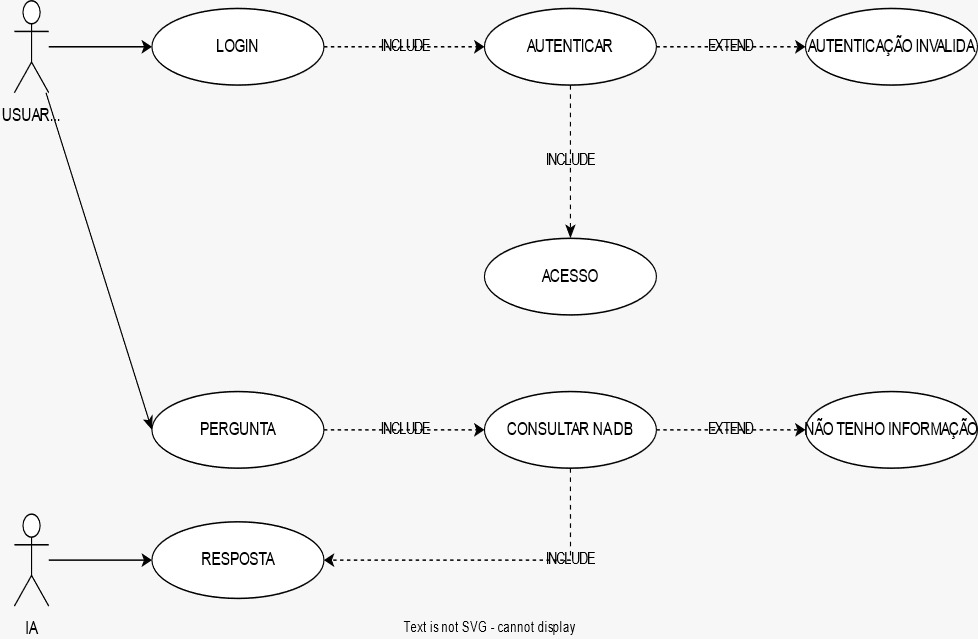
\includegraphics[height=8.5cm]{casodeuso.jpeg}
    \caption{Diagrama de caso de uso do sistema MySupport AI}
    \label{fig:caso-de-uso}
\end{figure}


\subsection{Linguagem de programação}
\begin{itemize}
    \item Python – Flask
    \item JavaScript
    \item HTML
    \item CSS
\end{itemize}
\subsection{Banco de dados}
\begin{itemize}
    \item MongoDB.
\end{itemize}
\subsection{Outras ferramentas de desenvolvimento}
\begin{itemize}
    \item Premier, VScode, Canva, Ilustrator e Figma.
\end{itemize}

\section{REQUISITOS NÃO FUNCIONAIS}
\begin{itemize}
    \item Desempenho: O sistema deve ser altamente responsivo, capaz de lidar com picos de carga durante os horários de maior uso. O tempo de resposta para operações críticas, como abertura de chamados, resposta do chatbot e atualização do status, deve ser inferior a 2 segundos.
    \item Usabilidade: A interface do usuário deve ser intuitiva e organizada, permitindo fácil navegação por usuários com diferentes níveis de familiaridade com tecnologia. O design deve seguir os princípios de usabilidade, priorizando acessibilidade, clareza e consistência visual para reduzir a curva de aprendizado.
    \item Segurança: O sistema deve aplicar medidas robustas para proteger dados sensíveis dos usuários, incluindo informações pessoais e conteúdos dos chamados. Deve haver autenticação e controle de acesso baseado em níveis de permissão (usuário, atendente, administrador). Toda transmissão e armazenamento de dados sensíveis deve utilizar criptografia forte (como TLS para transmissão e AES para armazenamento).
    \item Confiabilidade e Disponibilidade: O sistema deve apresentar alta confiabilidade, com no máximo 0,1\% de tempo de inatividade durante o horário comercial. Deve contar com planos de contingência e backups regulares para garantir a continuidade das operações em caso de falhas.
    \item Escalabilidade: O sistema deve ser escalável para acompanhar o crescimento da demanda, suportando um número crescente de usuários simultâneos e chamados abertos. A arquitetura deve permitir expansão simples tanto em software (módulos adicionais) quanto em infraestrutura (mais servidores, containers etc.).
    \item Compatibilidade: O sistema deve ser compatível com navegadores modernos e sistemas operacionais diversos, incluindo Windows, macOS e Linux. Deve também garantir integração eficiente com periféricos, como câmeras para videoconferência, microfones e dispositivos móveis.
    \item Manutenibilidade: A estrutura do código deve ser modular, favorecendo a manutenção e a adição de novos recursos. Toda a aplicação deve ser acompanhada de documentação técnica clara e completa.
    \item Portabilidade: O sistema deve ser facilmente implantável em diferentes ambientes (nuvem, VPS, servidor local). Atualizações e migrações devem ser possíveis sem necessidade de reconfigurações complexas ou perda de dados.
\end{itemize}

\subsection{Tela de login.}
\begin{figure}[h!]
    \centering
    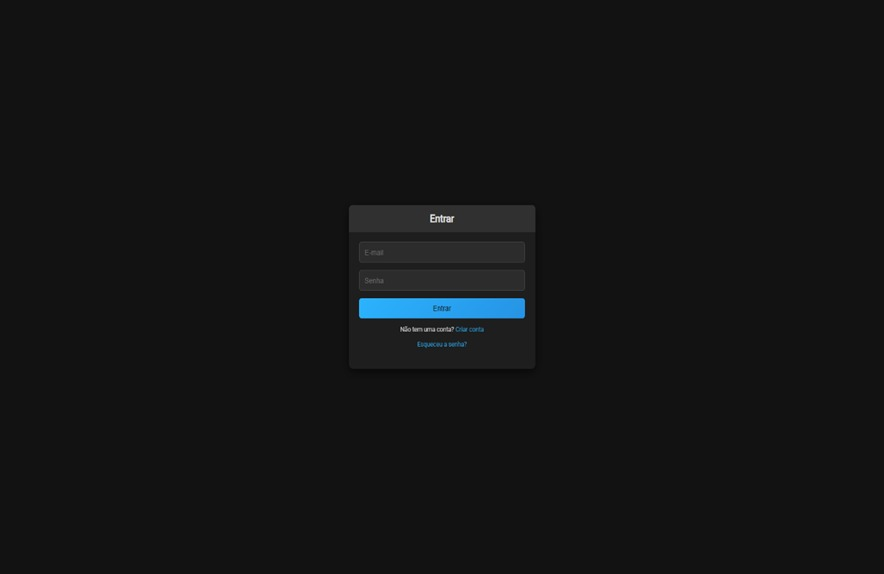
\includegraphics[height=10cm]{teladelogin.jpg}
    \caption{Tela de login do sistema MySupport AI}
    \label{fig:tela-de-login}
\end{figure}

\subsection{Cadastro de usuários.}
\begin{figure}[h!]
    \centering
    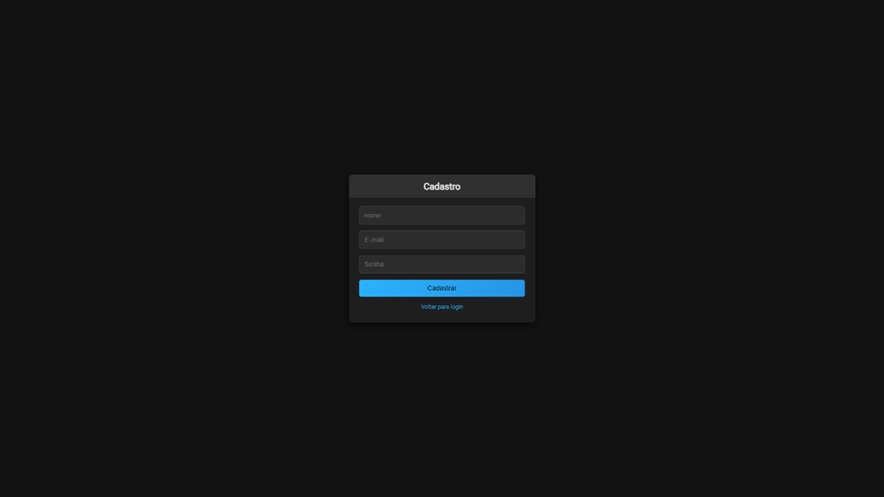
\includegraphics[height=8.7cm]{cadastrodeusuarios.jpg}
    \caption{Cadastro de usuários do sistema MySupport AI}
    \label{fig:cadastro-de-usuarios}
\end{figure}

\subsection{Redefinir senha.}
\begin{figure}[h!]
    \centering
    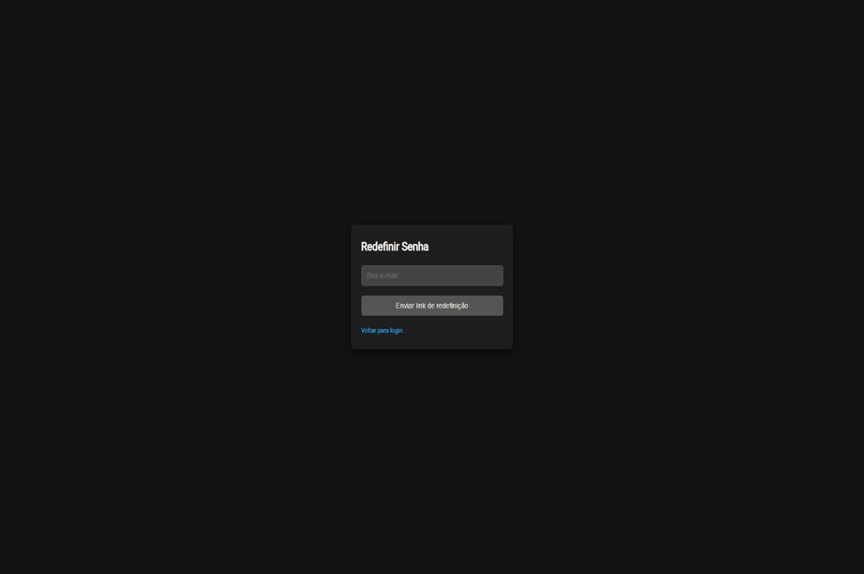
\includegraphics[height=10cm]{redefinirpass.jpg}
    \caption{Tela de redefinição de senha do sistema MySupport AI}
    \label{fig:redefinir-senha}
\end{figure}

\subsection{Read-me page.}
\begin{figure}[h!]
    \centering
    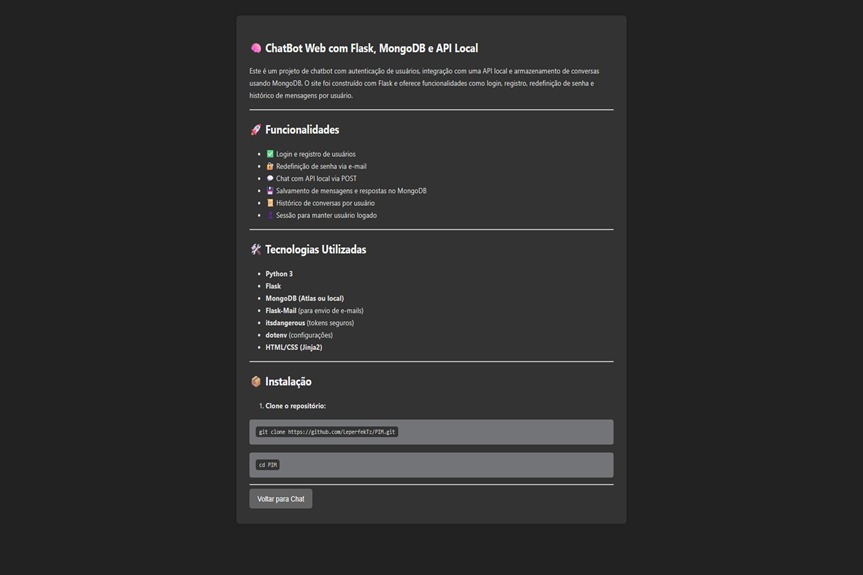
\includegraphics[height=8.7cm]{readme.jpg}
    \caption{Documentação (Read-me) do sistema MySupport AI}
    \label{fig:readme}
\end{figure}

\clearpage

\section{Conclusão}
O desenvolvimento do sistema de suporte com inteligência artificial proposto neste projeto visa modernizar e otimizar o atendimento ao cliente, oferecendo respostas rápidas, precisas e personalizadas por meio de um chatbot inteligente. A integração com tecnologias como Electron JS, Node.js e bancos de dados eficientes permite a criação de uma plataforma robusta, segura e escalável, que atende tanto às necessidades operacionais quanto às expectativas dos usuários.

Ao considerar requisitos funcionais e não funcionais de forma detalhada, o sistema garante não apenas funcionalidade, mas também desempenho, segurança, usabilidade e confiabilidade. Além disso, sua arquitetura modular facilita manutenções futuras e ampliações conforme o crescimento da empresa ou novas demandas surgirem.

Este projeto representa um passo importante rumo à automação inteligente do suporte técnico, contribuindo para a satisfação dos usuários e a eficiência operacional da organização.

\section{Materiais de referência}
\sloppy % Ajuda a evitar quebras ruins em URLs longas
\begin{samepage}
\noindent
\url{https://www.mongodb.com/}
\end{samepage}
\end{document}